\chapter[Correlation and regression]{Correlation and\\regression}

\section[Relation of mass and height]{In a dataset measuring people’s height and mass, let’s examine the relationship between height and mass.}



\begin{multicols}{2}
	\begin{enumerate}[a)]
	\item Based on the plot, what would you say about the linear relationship?

		\begin{itemize}
		\item direction: 	\hrulefill	
		\item strength: \hrulefill
		\end{itemize}
	
	\item The correlation coefficient calculated from the data is $r = 0.6556$.

	
	What does the \dots of the correlation coefficient indicate?
	
		\begin{itemize}
		\item absolute value: \hrulefill	% TODO
		\item sign: 	\hrulefill
		\end{itemize}

	\item How would you describe this linear relationship based on the correlation coefficient? \hrulefill	
	\item Why do we need to test whether the correlation coefficient is significant? \hrulefill	
	
		\columnbreak
			\begin{center}
		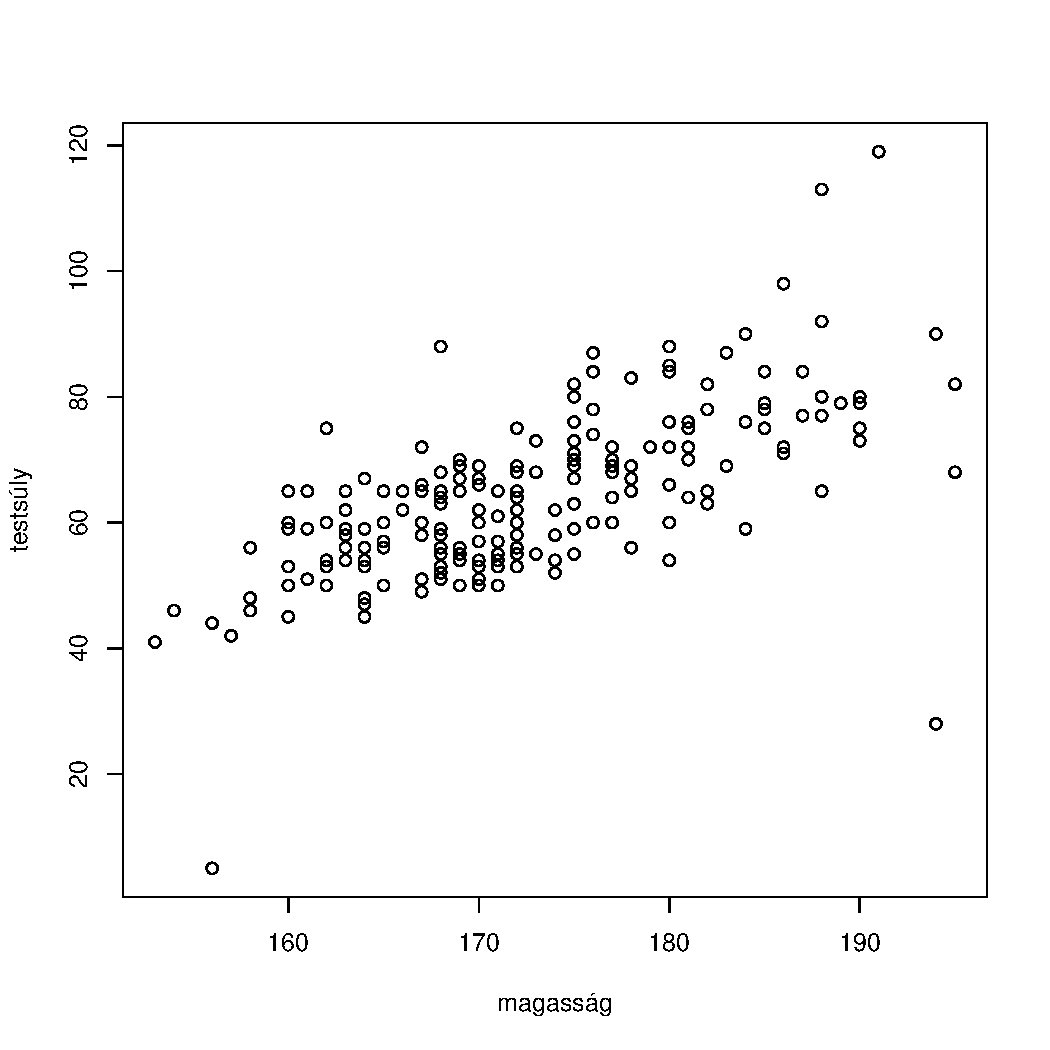
\includegraphics[width=0.48\textwidth]{Korrelacio-1}
		\end{center}
	\end{enumerate}
\end{multicols}

	
\subsection*{Significance test for the correlation coefficient ($n = 206$)}  
\begin{enumerate}[a)]\setcounter{enumi}{4}
\item Null hypothesis: \hrulefill		
	
	 Alternative hypothesis: \hrulefill		
\item t-value of the correlation: \hrulefill	
\item Degrees of freedom:	\hrulefill	 \quad Critical value: ($t_\alpha$): 	\hrulefill	
\item Decision and conclusion: \hrulefill		
\item The equation of the regression line: $y = 0,9698\cdot x - 103,147$ ($\textrm{mass} = 0,9698 \cdot \textrm{height}- 103,147$)

	Meaning: 	\hrulefill

	 What mass ''belongs'' to someone whose height is 160 cm, based on the regression line? \hrulefill	


\item Coefficient of determination

$$r^2 = \frac{ \textrm{squares}_{Regression} }{ \textrm{squares}_{Total} } = 0.4299$$

Meaning: 	\hrulefill
\subsection*{Find these values in the R output.}

\lstinputlisting[float=!h,frame=tblr]{Code/06-correlation1.txt}



\subsection*{Significance tests for the coefficients of the regression line}
\item Null hypothesis of the regression coefficient: \hrulefill\quad $t$-value: \hrulefill\quad	df: \hrulefill

$p$-value:	\hrulefill\quad significance:	\hrulefill\quad

\item Null hypothesis of the constant term: \hrulefill\quad $t$-value: \hrulefill\quad df: \hrulefill

$p$-value:	\hrulefill\quad significance:	\hrulefill\quad

\end{enumerate}
\clearpage




\section[Connection of money spent on alcohol and tobacco]{A British survey examined the connection of money spent on alcohol and tobacco in 10 different regions of GBR. The correlation coefficient of money spent on alcohol and tobacco is $r = 0.784$. Test whether this is significantly different from 0 at 5\% level. (\data{S:/R/alcohol.csv})}

\subsection*{Hand calculation}
\begin{enumerate}[a)]
\item H$_0$: \hrulefill		


 H$_A$: \hrulefill		
 
 Assumption(s): \hrulefill
\item $t$-value: \hrulefill\quad df:	\hrulefill	 \quad Critical value ($t_\alpha$): 	\hrulefill	
\item Decision: \hrulefill

	 Conclusion: \hrulefill

\subsection*{We ran the previous example in R. Interpret the results.}

\lstinputlisting[float=!h,frame=tblr]{Code/06-correlation2.txt}
\begin{flushright}
	\vspace{-18em}
	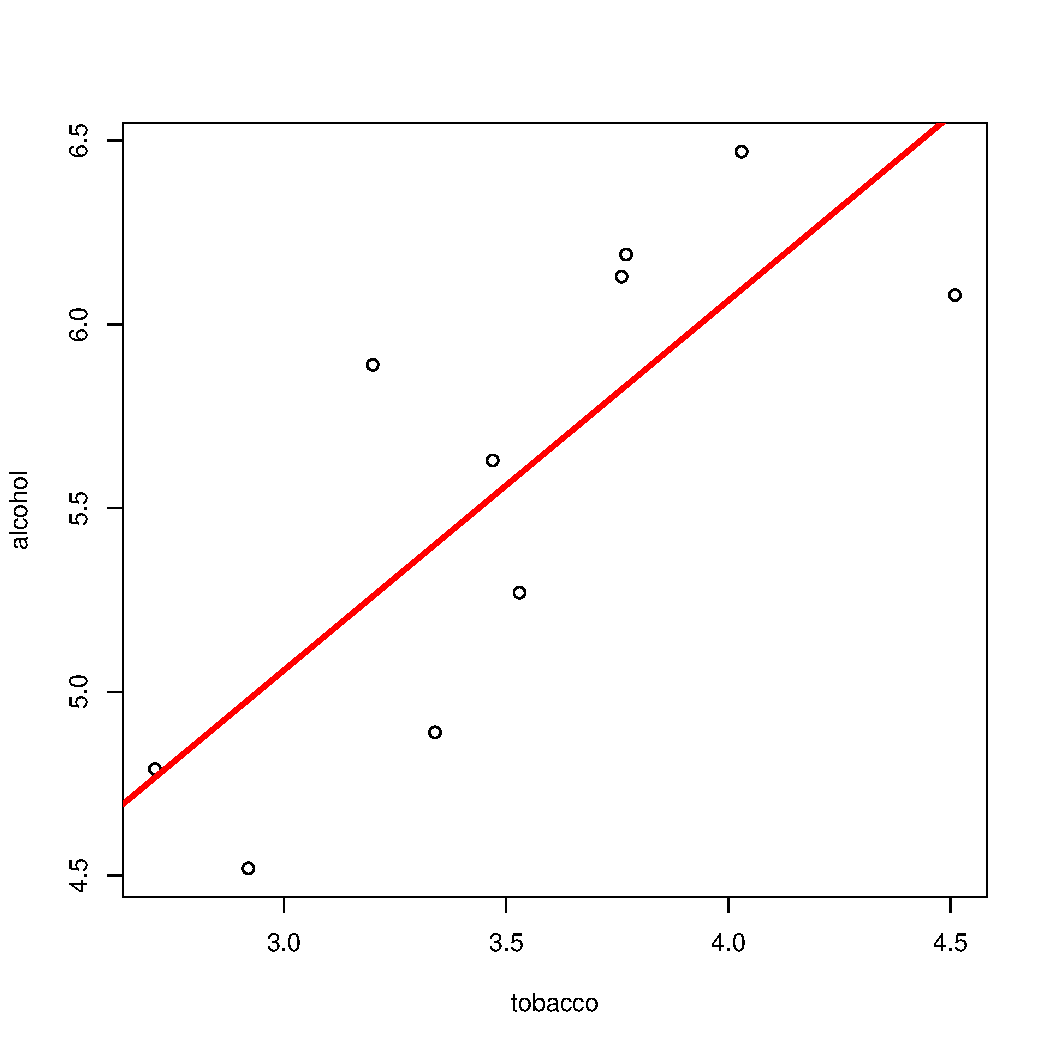
\includegraphics[width=0.3\textwidth]{Korrelacio-2}\hspace*{3em}
\end{flushright}

\item Correlation coefficient ($r$): \hrulefill\quad 	 Coefficient of determination $r^2$: \hrulefill
\item $t$:\hrulefill\quad df: \hrulefill\quad	 $p$-value:	\hrulefill
\item Conclusion to the direction and strength of the linear relationship: 	\hrulefill
\item Equation of the regression line: \hrulefill


\item Significance of the regression coefficients (use R to answer this question): \hrulefill
\end{enumerate}
\clearpage

\section{Is the correlation coefficient significantly different from 0 at 5\% level?}

 H$_0$: \hrulefill\quad H$_A$: \hrulefill		
\subsection{Based on $n = 5$ pairs of observations, the correlation coefficient is $r = 0.8$.}
\begin{enumerate}[a)]
\item $t$-value: \hrulefill\quad df:	\hrulefill	 \quad Critical value ($t_\alpha$): 	\hrulefill	
\item Decision: \hrulefill

	Interpretation (is there a contradiction?): \hrulefill
\end{enumerate}

\subsection{Based on $n = 500$ pairs of observations, the correlation coefficient is $r = 0.2$.}
\begin{enumerate}[a)]
%\item H$_0$: \hrulefill\quad H$_A$: \hrulefill		
\item $t$-value: \hrulefill\quad df:	\hrulefill	 \quad Critical value ($t_\alpha$): 	\hrulefill	
\item Decision: \hrulefill

	 Interpretation (is there a contradiction?): \hrulefill
\end{enumerate}

\subsection{Based on $n = 15$ pairs of observations, the correlation coefficient is $r = -0.8$.}

\begin{enumerate}[a)]
%\item H$_0$: \hrulefill\quad H$_A$: \hrulefill		
\item $t$-value: \hrulefill\quad df:	\hrulefill	 \quad Critical value ($t_\alpha$): 	\hrulefill	
\item Decision: \hrulefill

 Interpretation: \hrulefill
\end{enumerate}

\section{Practice with R}
\subsection{Open the \quest data file. Examine the relationship between \variable{height} and \variable{mass}. Create a scatter plot. }
\begin{enumerate}[a)]
\item Correlation coefficient $r$: \hrulefill\quad	 Coefficient of determination $r^2$:	 \hrulefill
\item % Correlation coefficient szignifikanciája
%
	 $t$: \hrulefill\quad	 df: \hrulefill\quad $p$:	 \hrulefill

 Decision: \hrulefill
%	Conclusion to the direction and strength of the linear relationship: \hrulefill
\item Equation of the regression line: \hrulefill
\item Significance of the regression coefficients: \hrulefill
\end{enumerate}

\subsection{Open the data file \data{anthropometrics.csv}! Examine the connection between the first and second measurement of weight. Create a scatter plot.}
%Készítsünk ábrát!
\begin{enumerate}[a)]
\item Correlation coefficient $r$: \hrulefill\quad	 Coefficient of determination $r^2$:	 \hrulefill
\item %Correlation coefficient szignifikanciája 
$t$: \hrulefill\quad	 df: \hrulefill\quad $p$:	 \hrulefill

 Decision: \hrulefill
%	Conclusion to the direction and strength of the linear relationship: \hrulefill
\item Equation of the regression line: \hrulefill
\item Significance of the regression coefficients: \hrulefill
\end{enumerate}

\subsection{ Open the data file \data{anthropometrics.csv}! Examine the linear association between height and hip circumference. Create a scatter plot.}
\begin{enumerate}[a)]
\item Correlation coefficient $r$: \hrulefill\quad	 Coefficient of determination $r^2$:	 \hrulefill
\item %Correlation coefficient szignifikanciája 
%
	 $t$: \hrulefill\quad	 df: \hrulefill\quad $p$:	 \hrulefill

 Decision: \hrulefill
\item Equation of the regression line: \hrulefill
\item Significance of the regression coefficients: \hrulefill
\end{enumerate}
